\documentclass[dvipdfmx,uplatex]{jsarticle}

%% Packages
\usepackage{graphicx,color,hyperref}
\usepackage{algorithm}
\usepackage{algorithmic}
\usepackage{url}
\usepackage{lscape}
\usepackage{mathtools}
\usepackage{here}
\usepackage{amsmath,amssymb,amsfonts}
\usepackage{amsthm}
\usepackage{tikz}
\usepackage{tcolorbox}
\usepackage{pxjahyper}

%% Theorem Styles
\newtheorem{theorem}{定理}
\newtheorem{proposition}{命題}
\newtheorem{cor}{系}
\newtheorem{definition}{定義}
\newtheorem{problem}{問題}
\theoremstyle{remark}
\newtheorem{remark}{注意}
\newtheorem{requirement}{条件}

%% Environment (Colorful Box)
\newenvironment{simplebox}{
    \begin{tcolorbox}[
        fonttitle=\bfseries,
    ]
}{
    \end{tcolorbox}
}

\newenvironment{method}[1]{
    \begin{tcolorbox}[
        colframe=green!50!black,
        colback=green!50!black!10!white,
        colbacktitle=green!50!black!40!white,
        coltitle=black,
        fonttitle=\bfseries,
        title={#1}
    ]
}{
    \end{tcolorbox}
}

\newenvironment{experiment}[1]{
    \begin{tcolorbox}[
        colframe=violet,
        colback=violet!10!white,
        colbacktitle=violet!40!white,
        coltitle=black,
        fonttitle=\bfseries,
        title={#1}
    ]
}{
    \end{tcolorbox}
}

\newenvironment{kansou}{
    \begin{tcolorbox}[
        colframe=brown,
        colback=brown!10!white,
        colbacktitle=brown!40!white,
        coltitle=black,fonttitle=\bfseries
    ]
}{
    \end{tcolorbox}
}

%% Title
\title{Combining Small Language Models and Large Language Models for Zero-Shot NL2SQL}
\author{\empty}
\date{\empty}

% https://gemini.google.com/app/b5ad0b088f9ba5db

%% Document body
\begin{document}
\maketitle

\begin{itemize}
    \item Link: \url{https://www.vldb.org/pvldb/vol17/p2750-fan.pdf}
    \item Conference: VLDB2024
    \item Citation: \cite{text2sql_with_slm_and_llm}
    \item Arxiv: \url{https://www.vldb.org/pvldb/vol17/p2750-fan.pdf}
\end{itemize}

\section{概要}
\begin{simplebox}
\begin{itemize}
    \item SLMとLLMを組み合わせて、Zero-ShotなNL2SQLを実現する手法を提案.
    \item SLMは、SQLスケッチを生成し、LLMがスケッチ中の情報を埋めることで、SQLクエリを生成する。
    \item この手法はZero-ShotなNL2SQL手法のこれまでのSOTAを上回る性能を示す。
\end{itemize}
\end{simplebox}

\section{背景}
\begin{simplebox}
\begin{itemize}
    \item この論文でいうZeroShotなNL2SQLとは、今対象としているデータベースに対するSQLクエリをプロンプトに含めない状態で、自然言語からSQLクエリを生成することを指す。
    \item 全く新しいデータベースに対するクエリを発行するときには、ZeroShotなNL2SQLが必要となる。
    \item SLMは、多くのNL2SQLサンプルで学習させることで、正確なSQLクエリを生成することができるが、自然言語から情報を取り出して推論することが難しい。
    \item LLMは自然言語の推論が得意であるが、正確なスキーマに基づくSQLクエリを生成するのが難しい。
    \item よってSLMにSQLの構文のみ生成させ、残りの自然言語から情報を取り出す部分をLLMに任せることで、正確なSQLを生成する。イメージは図\ref{fig:overview}の通りである。
\end{itemize}
\end{simplebox}

\begin{figure}
    \centering
    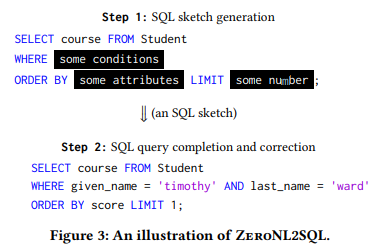
\includegraphics[width=0.5\textwidth]{img/text2sql-with-slm-and-llm/overview.png}
    \caption{提案手法の概要}
    \label{fig:overview}
\end{figure}

\section{手法}
\begin{method}{Overview}
\begin{enumerate}
    \item SLMがSQLスケッチを生成する、SQLスケッチは以下の情報で構成される。
    \begin{itemize}
        \item SELECT: 取得するカラム名
        \item FROM: 対象テーブル名
        \item Keywords: ORDER BY, GROUP BY, WHEREなどSQLに使われるキーワード、またSELECTなどサブクエリに使われるキーワードも含む。
    \end{itemize}
    \item LLMがSQLスケッチを受け取り、スケッチ中の情報を埋めることで、SQLクエリを生成する。
\end{enumerate}
\end{method}

\begin{method}{SQLスケッチの生成}
\begin{itemize}
    \item ここではSLMによるSQLスケッチの生成について説明する。
    \item SLMは、自然言語の質問とスキーマ情報を入力として、SQLスケッチを生成する。ただこれまでの手法で質問に含まれるカラム情報からカラムを選ぶことが多く、スキーマ情報が活用されていなかったため、次のようなエンコードをすることでスキーマ情報を活用する。
    \item 情報は次のようにエンコードされる: [INS] \textless question \textgreater : [Q] \textless database \textgreater : t0: \textless table0 \textgreater (c0: \textless column0 \textgreater , c1: \textless column1 \textgreater , ...), t1: \textless table1 \textgreater (c0: \textless column0 \textgreater , c1: \textless column1 \textgreater , ...), ... 
    \item このようにエンコードして、SELECT t0.c2のようにSQLスケッチを生成する。これをDatabase-Aware Serializationと呼ぶ。
    \item Question-Aware Aligner: またスケッチの生成においては(SELECT句, Keywords)の生成も行う。この生成はつぎのように行う。
    \begin{itemize}
        \item 考え得るすべてのSELECT句とKeywordsの組み合わせを列挙し、それをつぎのようにSLMにエンコードする: [CLS] user question: Q. our solution: SELECT${}_i$, Keywords${}_j$ [SEP]
        \item これをSLMに入力して、ベクトル表現$H$を得る。その後全結合層$FC()$を通して、$a_{ij} = \mathrm{sigmoid}(FC(H))$をスコアとする(文中には$\mathrm{softmax}$って書いてあるけど$\mathrm{sigmoid}$だと思う、$FC()$はおそらく出力が一次元)。 
    \end{itemize}
\end{itemize}
\end{method}

\begin{method}{SQLクエリの補完と修正}
\begin{itemize}
    \item SQLスケッチの不足部分をLLMで補完する、クエリの実行結果やデータベースの内容に基づいて、SQLクエリを段階的に修正していく。
    \item まずMulti-level matching strategyについて説明する。
    \begin{itemize}
        \item これは値の整合性を確保しつつ、LLMが正しい値を補完できるように支援するための手法である。
        \item カラム単位、テーブル単位、データベース単位でチェックを行っていき、それぞれのレベルでLLMが推論した値とマッチする(値が近い)ものがあった場合にそのレベルで終了する。
        \item 値が近いということを判定するには、例えば文字ベースの類似度計算、意味ベース(embedding)の類似度計算を行って判定する。
    \end{itemize}
    \item 上記の方法で生成したクエリから、よいSQLクエリを選ぶ。
    \begin{itemize}
        \item SQLクエリの選択の際のアイデアは、クエリの実行結果を考慮することである、すなわち「生成したクエリを投げてみて、実行結果が空であればそのクエリは不適切である」とみなす。
        \item 具体的にはMulti-level matching strategyで生成したクエリを実行して、結果が空でないものを選ぶ。 
    \end{itemize}
\end{itemize}
\end{method}

\section{実験結果}
\begin{experiment}{実験手法}
\begin{itemize}
    \item データセット: Spiderデータセットを用いて学習し、Dr.Spider, GeoQuery, KaggleDBQAの4つのデータセットで検証をした。
    \item 評価指標: LLMによって生成されるSQLクエリと答えのSQLクエリを実行してその結果が一致するときに正解とする指標; Execution Accuracy (EX) を用いた。
    \item ベースライン: 
    \begin{itemize}
        \item SLMベース: SMBOP, RESDSQL, LLaMA2
        \item LLMベース: Vanilla LLM, LLM + ICL(SQLクエリ例を与える)
    \end{itemize}
    \item モデル: 
    \begin{itemize}
        \item LLM: OpenIA API (gpt-3.5-turbo-0613, gpt-4-0613)
        \item スケッチ学習: T5-3B,
        \item Question-Aware Aligner: T5-3B
        \item SQL Query Completion: Senetence-Bert, GloVe辞書
    \end{itemize}
\end{itemize}
\end{experiment}

\begin{experiment}{実験結果}
\begin{itemize}
    \item 精度は表\ref{fig:experiment}に示す。
    \item オープンソースLM(SLMのことと思われる)を用いた実験結果
    \begin{itemize}
        \item SLM vs GPTだとGPTの方が平均性能では劣る
        \item ZeroNL2SQLによりGPTはSLM系モデルを上回る精度となる。
    \end{itemize}
    \item 商用LLMを用いた実験結果
    \begin{itemize}
        \item ZeroNL2SQL vs LLM+ICLだとZeroNL2SQLのほうが平均性能では上回る。
        \item コスト的な観点ではZeroNL2SQLはICL手法よりもトークン消費量が圧倒的に少ない。
        \item 速度面でもZeroNL2SQLはVanilla LLMに次いで高速である。
    \end{itemize}
\end{itemize}
\end{experiment}

\begin{figure}
    \centering
    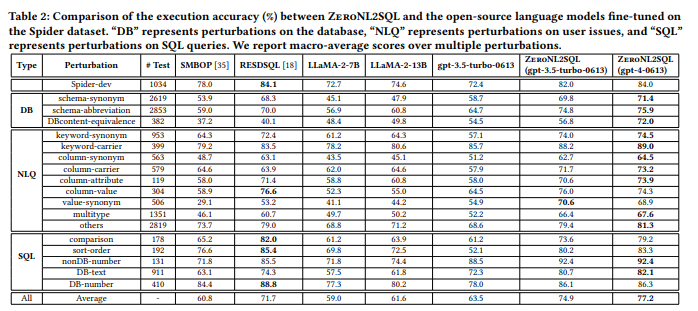
\includegraphics[width=0.9\textwidth]{img/text2sql-with-slm-and-llm/experiment.png}
    \caption{実験結果}
    \label{fig:experiment}
\end{figure}

\section{感想}
\begin{kansou}
\begin{itemize}
  \item テーブルスキーマのみでサンプルのSQLクエリ無しで自然言語からSQLクエリを生成するのは大変なのだなと思った。
  \item 新しいテーブルに対応するときにSQLクエリを用意しなくてよいのが良いところだと思う。
\end{itemize}
\end{kansou}

% \begin{figure}
%     \centering
%     
\includegraphics[width=0.5\textwidth]{img/image.png}
%     \caption{キャプション}
%     \label{fig:template}
% \end{figure}

\bibliographystyle{jplain}
\bibliography{template.bib}

\end{document}